\documentclass[11pt,]{article}
\usepackage[left=1in,top=1in,right=1in,bottom=1in]{geometry}
\newcommand*{\authorfont}{\fontfamily{phv}\selectfont}
\usepackage[]{mathpazo}


  \usepackage[T1]{fontenc}
  \usepackage[utf8]{inputenc}



\usepackage{abstract}
\renewcommand{\abstractname}{}    % clear the title
\renewcommand{\absnamepos}{empty} % originally center

\renewenvironment{abstract}
 {{%
    \setlength{\leftmargin}{0mm}
    \setlength{\rightmargin}{\leftmargin}%
  }%
  \relax}
 {\endlist}

\makeatletter
\def\@maketitle{%
  \newpage
%  \null
%  \vskip 2em%
%  \begin{center}%
  \let \footnote \thanks
    {\fontsize{18}{20}\selectfont\raggedright  \setlength{\parindent}{0pt} \@title \par}%
}
%\fi
\makeatother




\setcounter{secnumdepth}{0}

\usepackage{longtable,booktabs}

\usepackage{graphicx,grffile}
\makeatletter
\def\maxwidth{\ifdim\Gin@nat@width>\linewidth\linewidth\else\Gin@nat@width\fi}
\def\maxheight{\ifdim\Gin@nat@height>\textheight\textheight\else\Gin@nat@height\fi}
\makeatother
% Scale images if necessary, so that they will not overflow the page
% margins by default, and it is still possible to overwrite the defaults
% using explicit options in \includegraphics[width, height, ...]{}
\setkeys{Gin}{width=\maxwidth,height=\maxheight,keepaspectratio}

\title{Figures \& Tables: Seaweed extracts strongly structured microbial
communities associated with tomato and pepper roots and significantly
increased crop yield  }



\author{\Large Sébastien Renaut\textsuperscript{1,2},Jacynthe
Masse\textsuperscript{1,2}, Jeffrey P. Norrie\textsuperscript{3}, Bachar
Blal\textsuperscript{3} Mohamed Hijri\textsuperscript{1,2}\vspace{0.05in} \newline\normalsize\emph{}  }


\date{}

\usepackage{titlesec}

\titleformat*{\section}{\normalsize\bfseries}
\titleformat*{\subsection}{\normalsize\itshape}
\titleformat*{\subsubsection}{\normalsize\itshape}
\titleformat*{\paragraph}{\normalsize\itshape}
\titleformat*{\subparagraph}{\normalsize\itshape}





\newtheorem{hypothesis}{Hypothesis}
\usepackage{setspace}

\makeatletter
\@ifpackageloaded{hyperref}{}{%
\ifxetex
  \PassOptionsToPackage{hyphens}{url}\usepackage[setpagesize=false, % page size defined by xetex
              unicode=false, % unicode breaks when used with xetex
              xetex]{hyperref}
\else
  \PassOptionsToPackage{hyphens}{url}\usepackage[unicode=true]{hyperref}
\fi
}

\@ifpackageloaded{color}{
    \PassOptionsToPackage{usenames,dvipsnames}{color}
}{%
    \usepackage[usenames,dvipsnames]{color}
}
\makeatother
\hypersetup{breaklinks=true,
            bookmarks=true,
            pdfauthor={Sébastien Renaut\textsuperscript{1,2},Jacynthe
Masse\textsuperscript{1,2}, Jeffrey P. Norrie\textsuperscript{3}, Bachar
Blal\textsuperscript{3} Mohamed Hijri\textsuperscript{1,2} ()},
             pdfkeywords = {},  
            pdftitle={Figures \& Tables: Seaweed extracts strongly structured microbial
communities associated with tomato and pepper roots and significantly
increased crop yield},
            colorlinks=true,
            citecolor=blue,
            urlcolor=blue,
            linkcolor=magenta,
            pdfborder={0 0 0}}
\urlstyle{same}  % don't use monospace font for urls

% set default figure placement to htbp
\makeatletter
\def\fps@figure{htbp}
\makeatother

\usepackage[left]{lineno}
\linenumbers
\usepackage{caption}
\captionsetup{labelformat=empty}


% add tightlist ----------
\providecommand{\tightlist}{%
\setlength{\itemsep}{0pt}\setlength{\parskip}{0pt}}

\begin{document}
	
% \pagenumbering{arabic}% resets `page` counter to 1 
%
% \maketitle

{% \usefont{T1}{pnc}{m}{n}
\setlength{\parindent}{0pt}
\thispagestyle{plain}
{\fontsize{18}{20}\selectfont\raggedright 
\maketitle  % title \par  

}

{
   \vskip 13.5pt\relax \normalsize\fontsize{11}{12} 
\textbf{\authorfont Sébastien Renaut\textsuperscript{1,2},Jacynthe
Masse\textsuperscript{1,2}, Jeffrey P. Norrie\textsuperscript{3}, Bachar
Blal\textsuperscript{3} Mohamed Hijri\textsuperscript{1,2}} \hskip 15pt \emph{\small }   

}

}






\vskip 6.5pt


\noindent \doublespacing \newpage 

\begin{longtable}[]{@{}lllll@{}}
\caption{Table 1: summary of PERMANOVAs}\tabularnewline
\toprule
& fungi-soil & fungi-root & bacteria-soil & bacteria-root\tabularnewline
\midrule
\endfirsthead
\toprule
& fungi-soil & fungi-root & bacteria-soil & bacteria-root\tabularnewline
\midrule
\endhead
fertilization & 0.02*** & 0.08*** & 0.04*** & 0.07***\tabularnewline
planted & 0.21*** & NA & 0.13*** & NA\tabularnewline
species & 0.02*** & 0.26*** & 0.02*** & 0.52***\tabularnewline
fertilization:planted & 0.01** & NA & 0.02*** & NA\tabularnewline
fertilization:species & 0.01* & 0.04* & 0.03*** & 0.05***\tabularnewline
planted:species & 0.01 & NA & 0.01** & NA\tabularnewline
fertilization:planted:species & 0.01 & NA & 0.01* & NA\tabularnewline
\bottomrule
\end{longtable}

\(r^2\) (percentage of variance explained by the term in the model);
\emph{*p-value\textless{}0.05, **\textless{}0.005, ***\textless{}0.0005}

\newpage 

\includegraphics[width=6.25000in]{../figures/Figure_3_productivity.pdf}\\
\textbf{Figure 1: Measures of plant productivity. \emph{a} and \emph{b}
subscripts above boxplots denote significant differences according to
the fertilization treatment. Fold changes between the mean of the
control and fertilized plants were also noted for significant changes
(for pepper and tomato separately).}\\
\hspace*{0.333em}\\
\hspace*{0.333em}\\
\hspace*{0.333em}\\
\includegraphics[width=7.29167in]{../figures/Figure4_FAMILY_barplots_fungi.pdf}\\
\textbf{Figure 2: Barplots of the relative abundance of fungal ASVs for
fungi}\\
\hspace*{0.333em} ~\\
\hspace*{0.333em}\\
\includegraphics[width=7.29167in]{../figures/Figure4_FAMILY_barplots_bacteria.pdf}\\
\textbf{Figure 3: Barplots of the relative abundance of bacterial ASVs
for bacteria}\\
\hspace*{0.333em} ~\\
\hspace*{0.333em}\\
\includegraphics[width=6.25000in]{../figures/Figure5_alpha.pdf}\\
\textbf{Figure 4: Boxplot of \(a\)-diversity according to the treatment,
species and planting effect for fungal-root, fungal-soil, bacteria-soil
and bacteria-root. \emph{a} and \emph{b} subscripts above boxplots
denote significant differences.}\\
\hspace*{0.333em}\\
\hspace*{0.333em}\\
\hspace*{0.333em}\\
\includegraphics{../figures/fungi/Figure5f_rda.pdf}\\
\textbf{Figure 5: Canonical correspondence analyses for soil-fungi and
root-fungi. Samples were labeled and colored in gray (unfertilized) or
dark yellow (fertilized). Red crosses represent individual ASVs, while
red points represent the ten ASVs most closely associated with the three
productivity measures of root fresh weight, shoots fresh weight and
fruit number. Blue arrows are the four productivity measures used as
constraints in the ordinations.} ~\\
\hspace*{0.333em}\\
\hspace*{0.333em}\\
\includegraphics{../figures/bacteria/Figure6b_rda.pdf}\\
\textbf{Figure 6: Canonical correspondence analyses for soil-bacteria
and root-bacteria. Samples were labeled and colored in gray
(unfertilized) or dark yellow (fertilized). Red crosses represent
individual ASVs, while red points represent the ten ASVs most closely
associated with the three productivity measures of root fresh weight,
shoots fresh weight and fruit number. Blue arrows are the four
productivity measures used as constraints in the ordinations.} ~\\
\hspace*{0.333em}\\
\hspace*{0.333em} ~\\
\hspace*{0.333em} ~\\
\newpage 

\begin{longtable}[]{@{}lr@{}}
\caption{Table S1: Soil characteristics (in ppm unless specified
otherwise)}\tabularnewline
\toprule
Soil Characteristics & Average value\tabularnewline
\midrule
\endfirsthead
\toprule
Soil Characteristics & Average value\tabularnewline
\midrule
\endhead
pH & 6.01\tabularnewline
Conductivity (mmhos/cm) & 0.68\tabularnewline
Nitrate (N) & 62.40\tabularnewline
Ammonium & 0.09\tabularnewline
Phosphorus & 0.41\tabularnewline
Potassium & 29.30\tabularnewline
Calcium & 64.40\tabularnewline
Magnesium & 13.80\tabularnewline
Chloride & 28.50\tabularnewline
Sulfate & 19.30\tabularnewline
Sodium & 17.80\tabularnewline
Zinc & 0.12\tabularnewline
Manganese & 0.06\tabularnewline
Cooper & 0.81\tabularnewline
Iron & 0.90\tabularnewline
Aluminium & 1.66\tabularnewline
\bottomrule
\end{longtable}

~\\
\hspace*{0.333em}\\
\hspace*{0.333em}\\
\newpage    \includegraphics[width=6.77083in]{../figures/Figure1.png}\\
\textbf{Table S2: Randomized Split Block Experimental design}

~\\
\hspace*{0.333em}\\
\hspace*{0.333em}\\
\newpage   

\begin{longtable}[]{@{}ll@{}}
\caption{TableS3: Stella Maris® characteristics}\tabularnewline
\toprule
Stella Maris® characteristics & Average value\tabularnewline
\midrule
\endfirsthead
\toprule
Stella Maris® characteristics & Average value\tabularnewline
\midrule
\endhead
Appearance & Viscous Brownish-Black Liquid\tabularnewline
Odor & Marine Odor\tabularnewline
Solubility in water (\%) & 100\tabularnewline
pH & 7.4 - 8.2\tabularnewline
Carbohydrates & Alginic acid, Mannitol, Fucoidans\tabularnewline
Organic matter content (\%) & 13.0 - 16.0\tabularnewline
Total Nitrogen (N) (\%) & 0.1 - 0.6\tabularnewline
Available phosphate (P2O5) (\%) & \textless{} 0.2\tabularnewline
Soluble potash (K2O) (\%) & 5.0 - 7.0\tabularnewline
Sulphur (S) (\%) & 0.3 - 0.6\tabularnewline
Magnesium (Mg) (\%) & 0.05 - 0.15\tabularnewline
Calcium (Ca) (\%) & 0.05 - 0.15\tabularnewline
Sodium (Na) (\%) & 0.7 - 1.2\tabularnewline
Iron (Fe) (ppm) & 30 - 90\tabularnewline
Cooper (Cu) (ppm) & \textless{} 4\tabularnewline
Manganese (Mn) (ppm) & 3 - 11\tabularnewline
Boron (B) (ppm) & 20 - 40\tabularnewline
\bottomrule
\end{longtable}

~\\
\hspace*{0.333em}\\
\hspace*{0.333em}\\
\newpage 

\begin{longtable}[]{@{}lrrrr@{}}
\caption{Table S4: Summary of sequencing and bioinformatics
identification of ASVs}\tabularnewline
\toprule
& fungi-soil & fungi-root & bacteria-soil & bacteria-root\tabularnewline
\midrule
\endfirsthead
\toprule
& fungi-soil & fungi-root & bacteria-soil & bacteria-root\tabularnewline
\midrule
\endhead
No sequences (sum) & 976,000 & 309,000 & 920,000 &
535,000\tabularnewline
No sequences (mean) & 50,847 & 32,208 & 47,907 & 56,365\tabularnewline
No seq. filtered (mean) & 32,626 & 12,714 & 29,662 &
37,642\tabularnewline
No seq. filt. merged (mean) & 29,300 & 12,094 & 14,060 &
30,706\tabularnewline
No seq. filt. merg. no chimeras (mean) & 25,476 & 9,849 & 13,521 &
30,408\tabularnewline
No samples & 192 & 96 & 192 & 96\tabularnewline
No samples trimmed & 189 & 81 & 192 & 95\tabularnewline
No ASVs (sum) & 6,112 & 845 & 9,352 & 2,023\tabularnewline
No ASVs trimmed (sum) & 413 & 106 & 811 & 325\tabularnewline
ASV per sample (mean) & 176 & 37 & 269 & 92\tabularnewline
\bottomrule
\end{longtable}

~\\
\hspace*{0.333em}\\
\hspace*{0.333em}
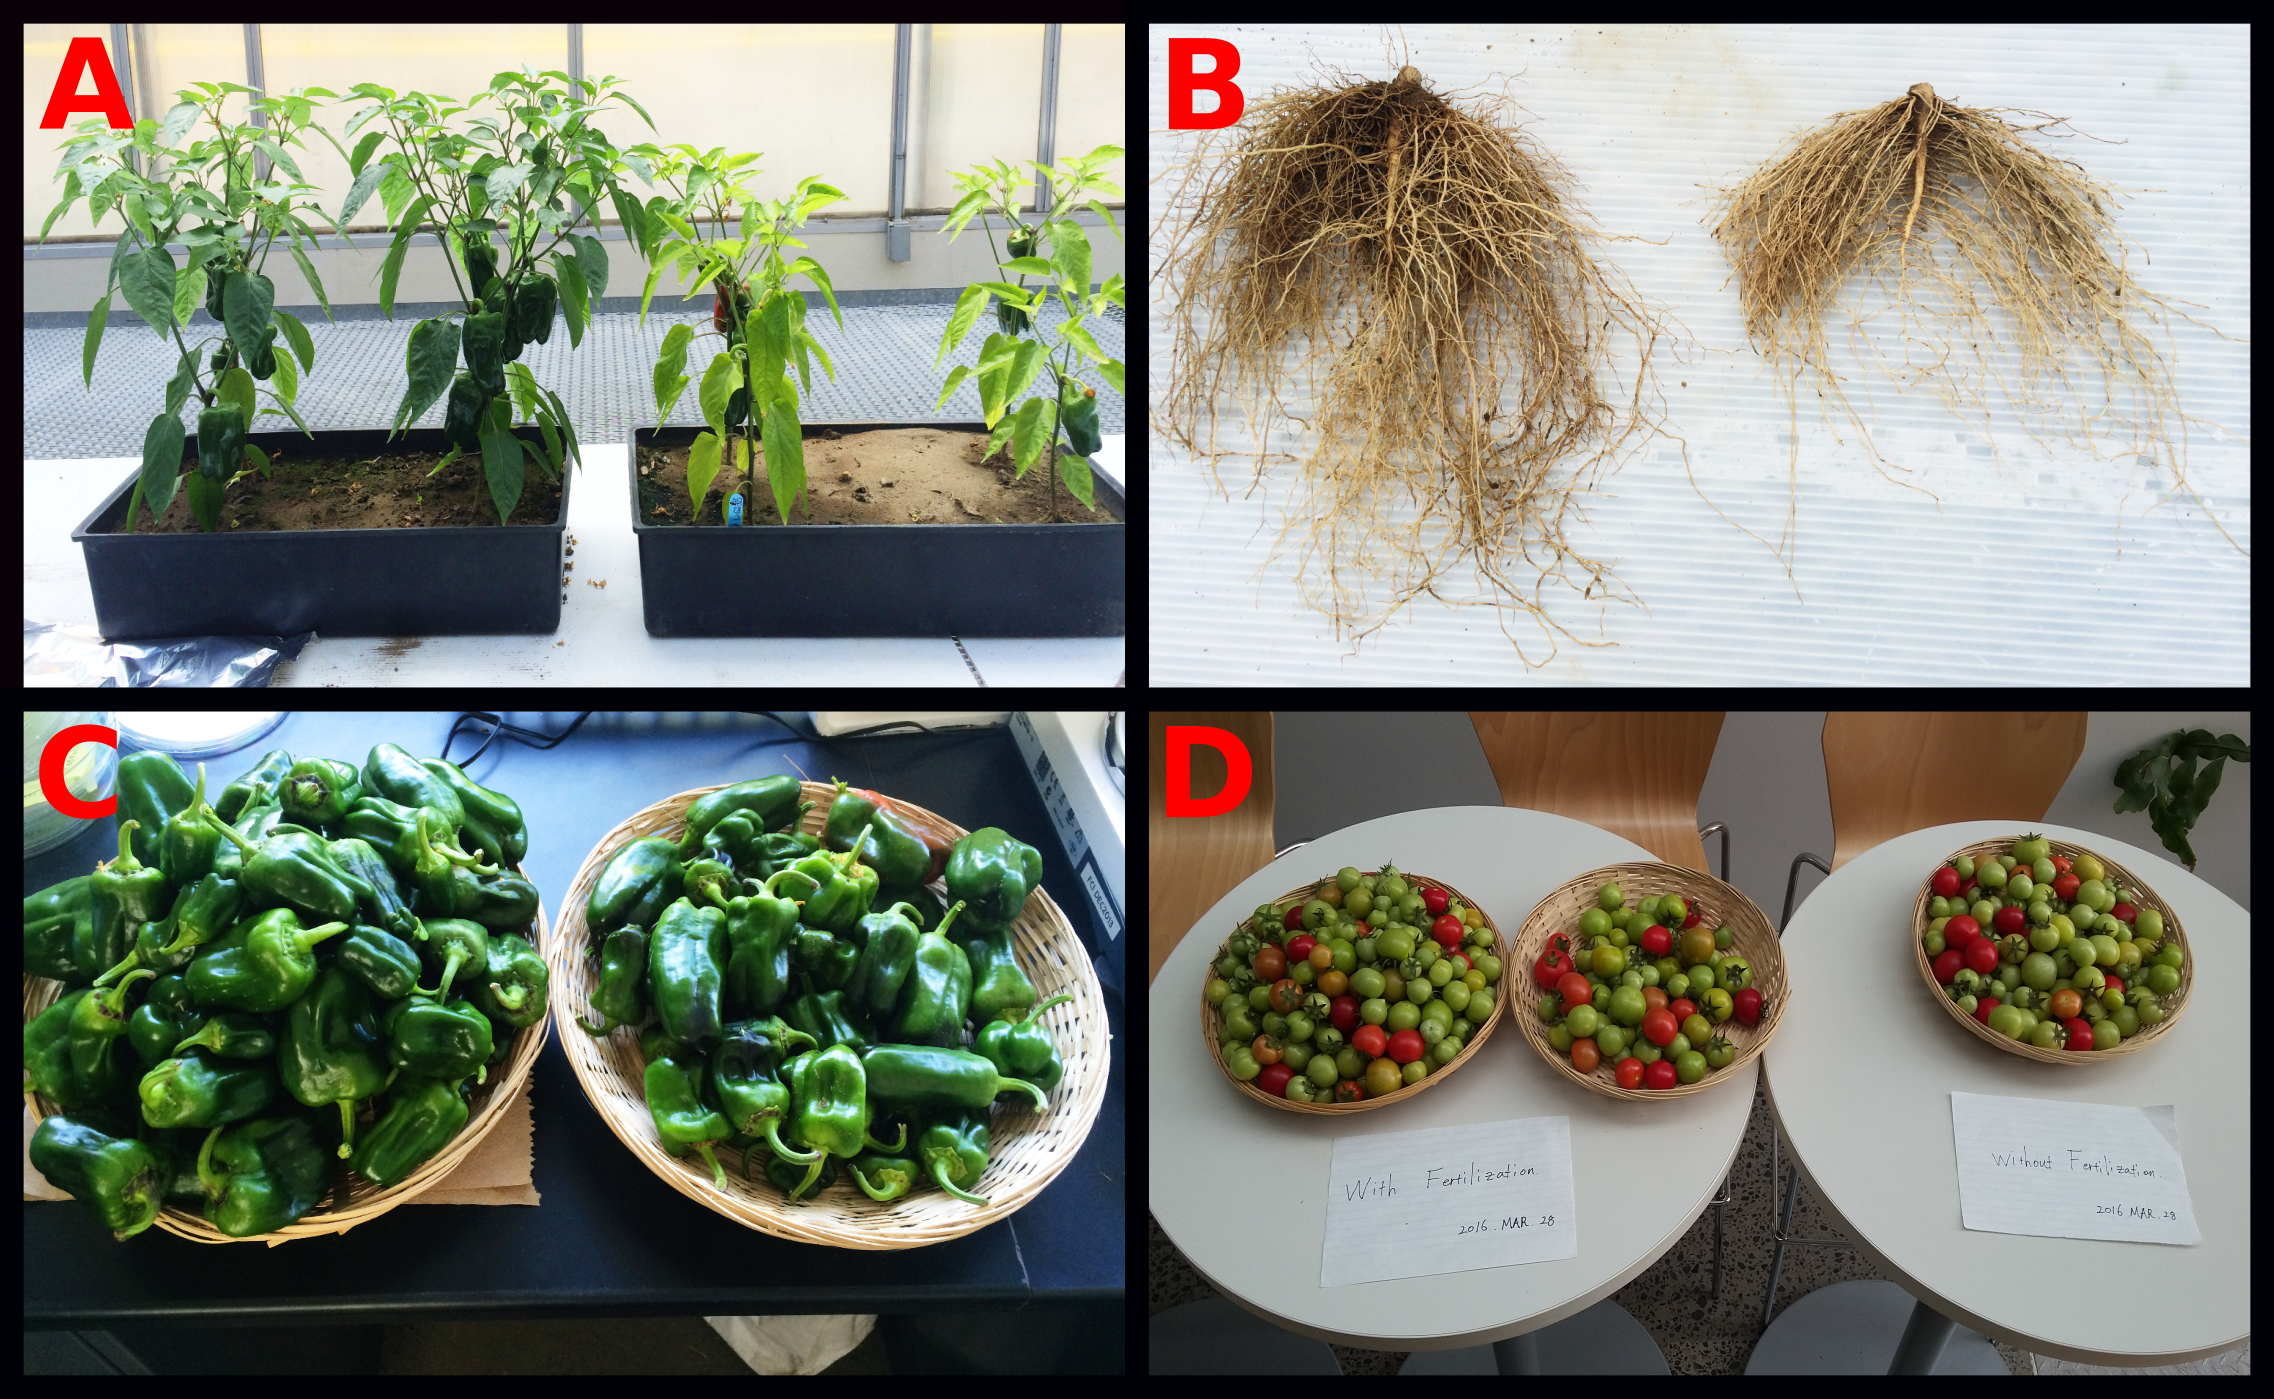
\includegraphics[width=5.20833in]{../figures/Figure_2_photos_productivity.png}\\
\textbf{Figure S1: Plant productivity. Photos were taken at the end of
the experimental treatment. In each photo, fertilized plants are on the
left. A: pepper shoots, B: pepper roots, C: pepper fruits and D: tomato
fruits.}\\
\hspace*{0.333em}\\
\hspace*{0.333em}\\
\hspace*{0.333em}\\
\includegraphics{../figures/fungi/Figure7_fungi_tree.pdf}\\
\textbf{Figure S2: Neighbor-Joining trees of candidates ASVs (fungi)
positively associated with productivity measures. The most accurate
taxonomy assigned according to the RDP bayesian classifier (form Phylum
to species) was added as tip labels.} ~\\
\hspace*{0.333em}\\
\hspace*{0.333em}\\
\includegraphics{../figures/bacteria/Figure7_bacteria_tree.pdf}\\
\textbf{Figure S3: Neighbor-Joining trees of candidates ASVs (bacteria)
positively associated with productivity measures. The most accurate
taxonomy assigned according to the RDP bayesian classifier (form Phylum
to species) was added as tip labels.} ~\\
\hspace*{0.333em}\\
\hspace*{0.333em}




\newpage
\singlespacing 
\end{document}
